% Chapter Template

\chapter{Background Knowledge} % Main chapter title

\label{Chapter3} % Change X to a consecutive number; for referencing this chapter elsewhere, use \ref{ChapterX}

\lhead{Chapter 3. \emph{Background Knowledge}} % Change X to a consecutive number; this is for the header on each page - perhaps a shortened title

%------------------------------------------------------------------
%	SECTION 1
%------------------------------------------------------------------

\section{Histogram Equalization of Gray-scale.}\label{sec:3.1}

Histogram is a graphical representation of the intensity distribution of an image. It quantifies the number of pixels for each intensity value considered.
\begin{figure}[t]
	\centering
	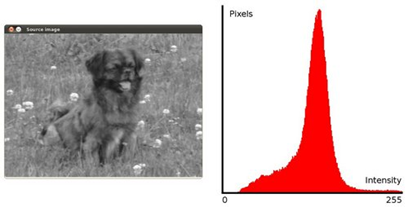
\includegraphics[scale=1]{f301.png}
	\caption{Original image and histogram}
	\label{fig:f301}
\end{figure}
Histogram equalization is a method that improves the contrast in an image, in order to stretch out the intensity range. To make it clearer, from Figure \ref{fig:f301}, the pixels seem clustered around the middle of the available range of intensities.What Histogram Equalization does is to stretch out this range. Take a look at the Figure \ref{fig:f302}: The green circles indicate the underpopulated intensities. After applying the equalization, the result is shown in a histogram in the Figure \ref{fig:f302} in the center. The resulting image is shown in the Figure \ref{fig:f302} at the right. Equalization implies mapping one distribution (the given histogram) to another distribution (a wider and more uniform distribution of intensity values) so the intensity values are spreaded over the whole range.


\begin{figure}[t]
	\centering
	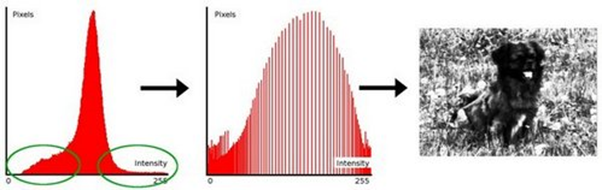
\includegraphics[scale=0.8]{f302.png}
	\caption{Gray-scale image equalization and histogram}
	\label{fig:f302}
\end{figure}

To accomplish the equalization effect, the remapping should be the \textit{cumulative distribution function (cdf)}. For the histrogram H(i), its \textit{cumulative distribution H'(i) is:}
\begin{align}
	H'(i) &= \sum_{0<=j<i}H(j)
\end{align}
Where i and j refer to an intensity value in horizontal x-axis.To use this as a remapping function, we have to normalize H'(i) such that the maximum value is 255 (or the maximum value for the intensity of the image). From the Figure 3.2, the cumulative function is shown in Figure \ref{fig:f303}.
\begin{figure}[t]
	\centering
	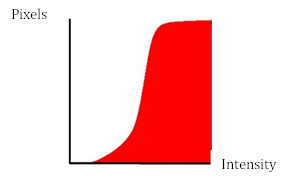
\includegraphics[scale=1]{f303.png}
	\caption{Maximum values for the intensity of the image}
	\label{fig:f303}
\end{figure}
Finally, using a simple remapping procedure to obtain the intensity values of the equalized image:
\begin{align}
	equalized(x,y) &= H'(src(x,y)) 
\end{align}
Where \textit{equalized(x,y)} is a function which performs equalization and \textit{src(x,y)} is a source image, x and y represent intensity values and pixels in sequence. 

%------------------------------------------------------------------
%	SECTION 2
%------------------------------------------------------------------

\section{Otsu Thresholding}\label{sec:3.2}
The thresholding function is typically used to get a binary image out of a gray-scale image or for removing a noise. There are several types of thresholding some of them are shown as in Figure \ref{fig:f304}.

Normally, threshold value is set manually. However, there is an algorithm that can compute the threshold value automatically, such as Otsu's algorithm.

Otsu's thresholding method involves iterating through all the possible threshold values and calculating a measure of spread for the pixel levels each side of the threshold, i.e. the pixels that either falls in foreground or background. The aim is to find the threshold value where the sum of foreground and background spreads is at its minimum.

\begin{figure}
	\centering
	\begin{subfigure}[b]{0.3\textwidth}
		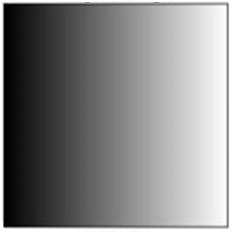
\includegraphics[width=\textwidth]{f304a.png}
		\caption{}
	\end{subfigure}%
	~ %add desired spacing between images, e. g. ~, \quad, \qquad, \hfill etc.
	%(or a blank line to force the subfigure onto a new line)
	\begin{subfigure}[b]{0.3\textwidth}
		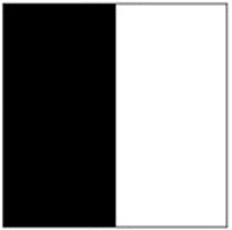
\includegraphics[width=\textwidth]{f304b.png}
		\caption{}
	\end{subfigure}
	~ %add desired spacing between images, e. g. ~, \quad, \qquad, \hfill etc.
	%(or a blank line to force the subfigure onto a new line)
	\begin{subfigure}[b]{0.3\textwidth}
		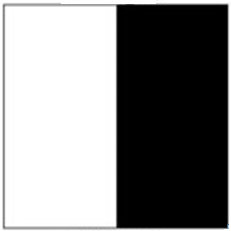
\includegraphics[width=\textwidth]{f304c.png}
		\caption{}
	\end{subfigure}
	\begin{subfigure}[b]{0.3\textwidth}
		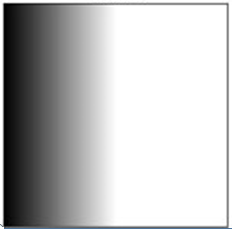
\includegraphics[width=\textwidth]{f304d.png}
		\caption{}
	\end{subfigure}
	\begin{subfigure}[b]{0.3\textwidth}
		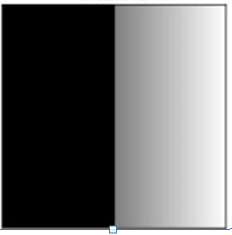
\includegraphics[width=\textwidth]{f304e.png}
		\caption{}
	\end{subfigure}
	\begin{subfigure}[b]{0.3\textwidth}
		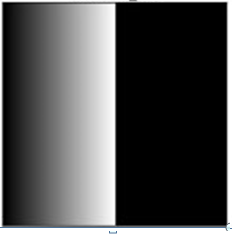
\includegraphics[width=\textwidth]{f304f.png}
		\caption{}
	\end{subfigure}
	\caption{(a) An original image (b) Binary image (c) Binary inverted image (d) Threshold truncated image (e) Threshold to zero image (f) Threshold to zero inverted image}\label{fig:f304}
\end{figure}
The algorithm will be demonstrated using the simple 6x6 pixels shown in Figure \ref{fig:f305}. The histogram for this image is shown on its right. To simplify the explanation, only 6 grey-scale levels are used.
\begin{figure}[t]
	\centering
	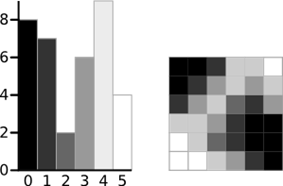
\includegraphics[scale=0.7]{f305.png}
	\caption{Histogram}
	\label{fig:f305}
\end{figure}

The calculations for finding the foreground and background variances for a single threshold as it set to 3. 

Finding variances of background, it start from finding means value of background. The mean $(\mu_{b})$ is an average of multiplications between intensity values and its number pixels. Consider Figure \ref{fig:f306}, horizontal x-axis represents intensity values and vertical y-axis represents number pixels. It shows intensity values which less than the threshold value. After the mean is calculated, the variance will be calculated. It is an average of multiplications between square of difference mean and the number pixels. Where the difference mean are difference between an intensity values, relate with the number pixels, and the mean value.
\begin{figure}[t]
	\centering
	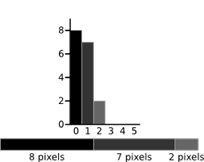
\includegraphics[scale=1]{f306}	
	\caption{Background}
	\label{fig:f306}
\end{figure}
\begin{align}
	W_{b} &= \frac{8+7+2}{36} &= 0.4722 \label{eq:w_b}\\
	\mu_{b} &= \frac{(0*8)+(1*7)+(2*2)}{17} &= 0.6471 \label{eq:mu_b}\\	
	\sigma_{b}^2 &= \frac{((0-0.6471)^2*8)*((1-0.6471)^2*7)+((2-0.6471)^2*2)}{17} &= 0.4637\label{eq:sig_b}
\end{align}

Finding variances of foreground, it start from finding means value of foreground. The mean $(\mu_{f})$ is an average of multiplications between intensity values and its number pixels. Consider Figure \ref{fig:f307} horizontal x-axis represents intensity values and vertical y-axis represents number pixels. It shows intensity values which more than the threshold value. After the mean is calculated, the variance will be calculated. It is an average of multiplications between square of difference mean and the number pixels. Where the difference mean are difference between an intensity values, relate with the number pixels, and the mean value.
	
\begin{figure}[t]
	\centering
	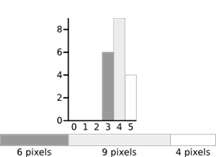
\includegraphics[scale=1]{f307.png}	
	\caption{Foreground}
	\label{fig:f307}
\end{figure}
\begin{align}
	W_{f} &= \frac{6+9+4}{36} &= 0.5278 \label{eq:w_f}\\
	\mu_{f} &= \frac{(3*6)+(4*9)+(5*4)}{19} &= 3.8947 \label{eq:mu_f}\\	
	\sigma_{f}^2 &= \frac{((3-3.8947)^2*6)*((4-3.8947)^2*9)+((5-3.8947)^2*4)}{19} &= 0.5152\label{eq:sig_f}
\end{align}	

The next step is to calculate the Within-Class Variance $(\sigma_{w}^2)$. This is simply the sum of the two variances, i.e. background variance (\ref{eq:sig_b}) , foreground variance (\ref{eq:sig_f}), multiplied by their associated weights. Note that, the weights are average of intensity, i.e. background weight equation (\ref{eq:w_b}), foreground weight equation (\ref{eq:w_f}).
\begin{align}
	\sigma_{w}^2 &= W_{b}\sigma_{b}^2 + W_{f}\sigma_{f}^2\\
	&=0.4722*0.4637+0.5278*0.5152\nonumber\\
	&=0.4909\label{eq:sumWeight}
\end{align}
This final value is the sum of weighted variances, equation (\ref{eq:sumWeight}), for the threshold value 3. This same calculation needs to be performed for all the possible threshold values 0 to 5. Figure \ref{fig:f308} shows the results for these calculations. The highlighted column shows the values for the threshold calculated at equation (\ref{eq:sumWeight}). 
\begin{figure}[t]
	\centering
	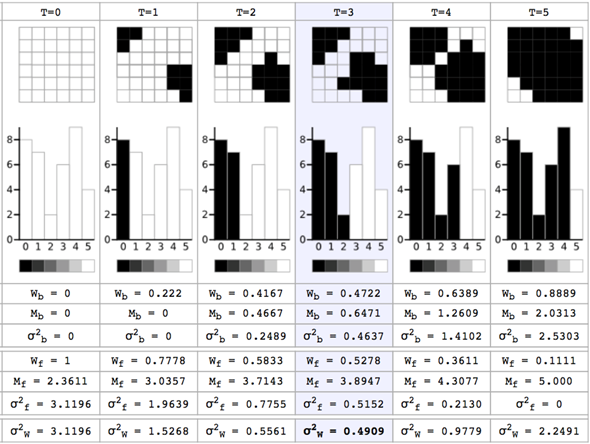
\includegraphics[scale=1]{f308.png}
	\caption{The results}
	\label{fig:f308}
\end{figure}
It can be seen that for the threshold equal to 3, as well as being used for the example, also has the lowest sum of weighted variances. Therefore, this is the final selected threshold. All pixels with a level less than 3 are background, all those with a level equal to or greater than 3 are foreground. The result of Otsu's method with threshold equals to 3 is shown in Figure \ref{fig:f309}. It can be seen that this method shows a good result in separation of foreground and background.
\begin{figure}[t]
	\centering
	
\includegraphics[scale=1]{f309.png}
	\caption{The threshold value}
	\label{fig:f309}
\end{figure}
%------------------------------------------------------------------
%	SECTION 3
%------------------------------------------------------------------

\section{RGB to Grey-Scale Image Conversion}
Normally, an input image is in RGB format. However, in order to perform image processing techniques, the RGB image is required to be converted into a gray-scale image. There are several methods to perform this conversion. In MATLAB the following conversion is used by forming a weighted sum of the R, G, and B components:
\begin{equation}
	0.2989 * R + 0.5870 * G + 0.1140 * B
\end{equation}
Consider an RGB image is shown in Figure \ref{fig:f3010a}. When apply the previous formula to convert it to the gray-scale image, the result is shown in Figure \ref{fig:f3010b}.
\begin{figure}
	\centering
	\begin{subfigure}[b]{0.3\textwidth}
		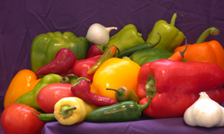
\includegraphics[width=\textwidth]{f3010a.png}
		\caption{}\label{fig:f3010a}
	\end{subfigure}
	\begin{subfigure}[b]{0.3\textwidth}
		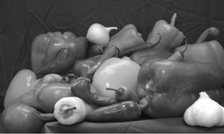
\includegraphics[width=\textwidth]{f3010b.png}
		\caption{}\label{fig:f3010b}
	\end{subfigure}
	\caption{(a) An original image (b) RGB to gray-scale image conversion result}
\end{figure}

%------------------------------------------------------------------
%	SECTION 4
%------------------------------------------------------------------

\section{Adaptive Histogram Equalization}\label{sec:3.4}
This technique is used to improve contrast in images. It differs from ordinary histogram equalization in the respect that the adaptive method computes several histograms, each corresponding to a distinct section of the image, and uses them to redistribute the lightness values of the image. It is therefore suitable for improving the local contrast of an image and bringing out more detail.
\begin{figure}
	\centering
	\begin{subfigure}[b]{0.3\textwidth}
		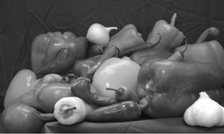
\includegraphics[width=\textwidth]{f3010b.png}
		\caption{}\label{fig:f3011a}
	\end{subfigure}
	\begin{subfigure}[b]{0.3\textwidth}
		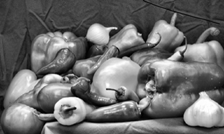
\includegraphics[width=\textwidth]{f3011b.png}
		\caption{}\label{fig:f3011b}
	\end{subfigure}
	\caption{(a) An original image (b) RGB to gray-scale image conversion result}\label{fig:f3011}
\end{figure}
Consider Figure \ref{fig:f3011} illustrate the differentiation of gray-scale image. An input image is shown in Figure \ref{fig:f3011a}. Figure \ref{fig:f3011b}, enhanced the contrast of the gray-scale image by transforming the values using contrast-limited adaptive histogram. 

More differentiation detail of enhancing the contrast of the gray-scale image is shown in Figure \ref{fig:f3012}. It illustrate comparing with the histogram differentiation between the gray-scale image and the enhanced contrast of gray-scale image. Figure \ref{fig:f3012a} represents to the gray-scale image before uses the contrast-limited adaptive histogram. Figure \ref{fig:f3012b} represents to the gray-scale image after uses the contrast-limited adaptive histogram.
\begin{figure}
	\centering
	\begin{subfigure}[b]{0.4\textwidth}
		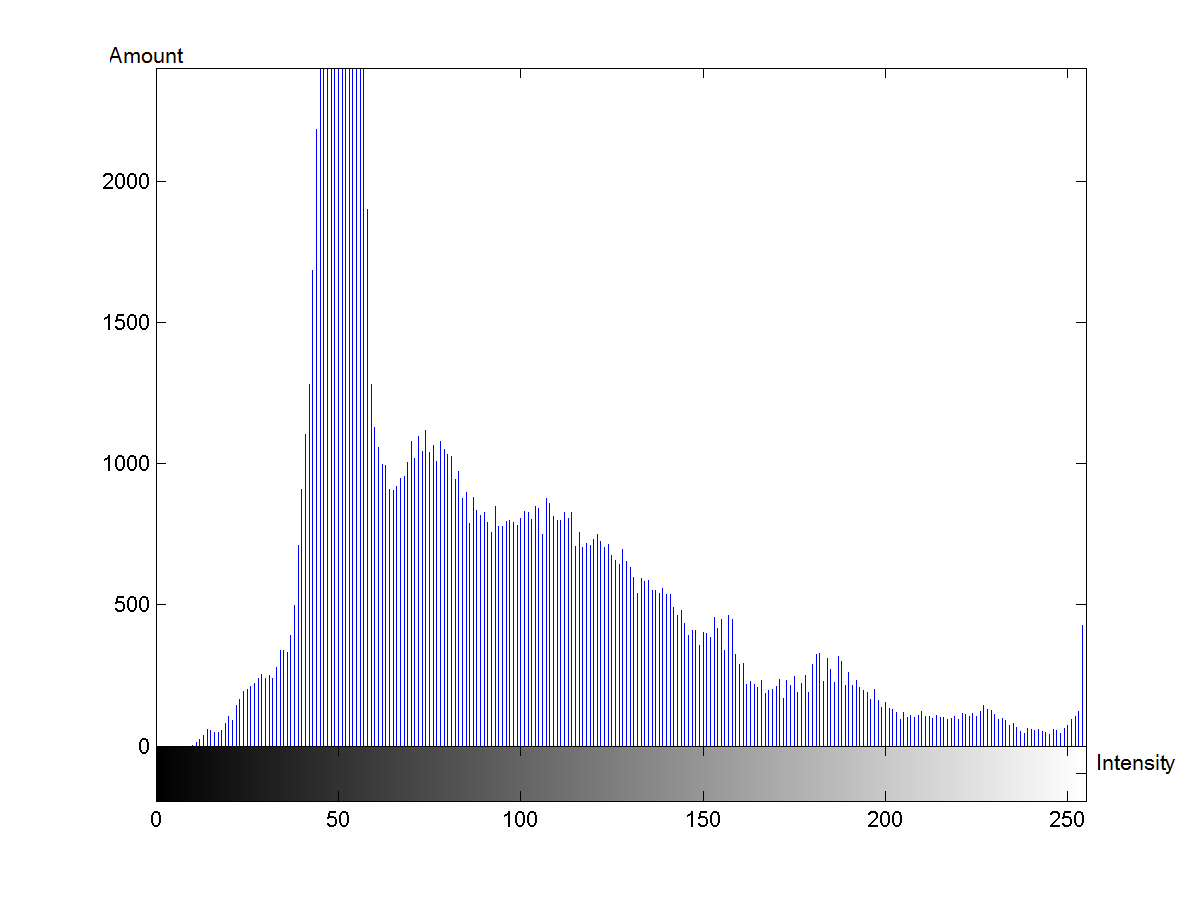
\includegraphics[width=\textwidth]{f3012a.png}
		\caption{}\label{fig:f3012a}
	\end{subfigure}
	\begin{subfigure}[b]{0.4\textwidth}
		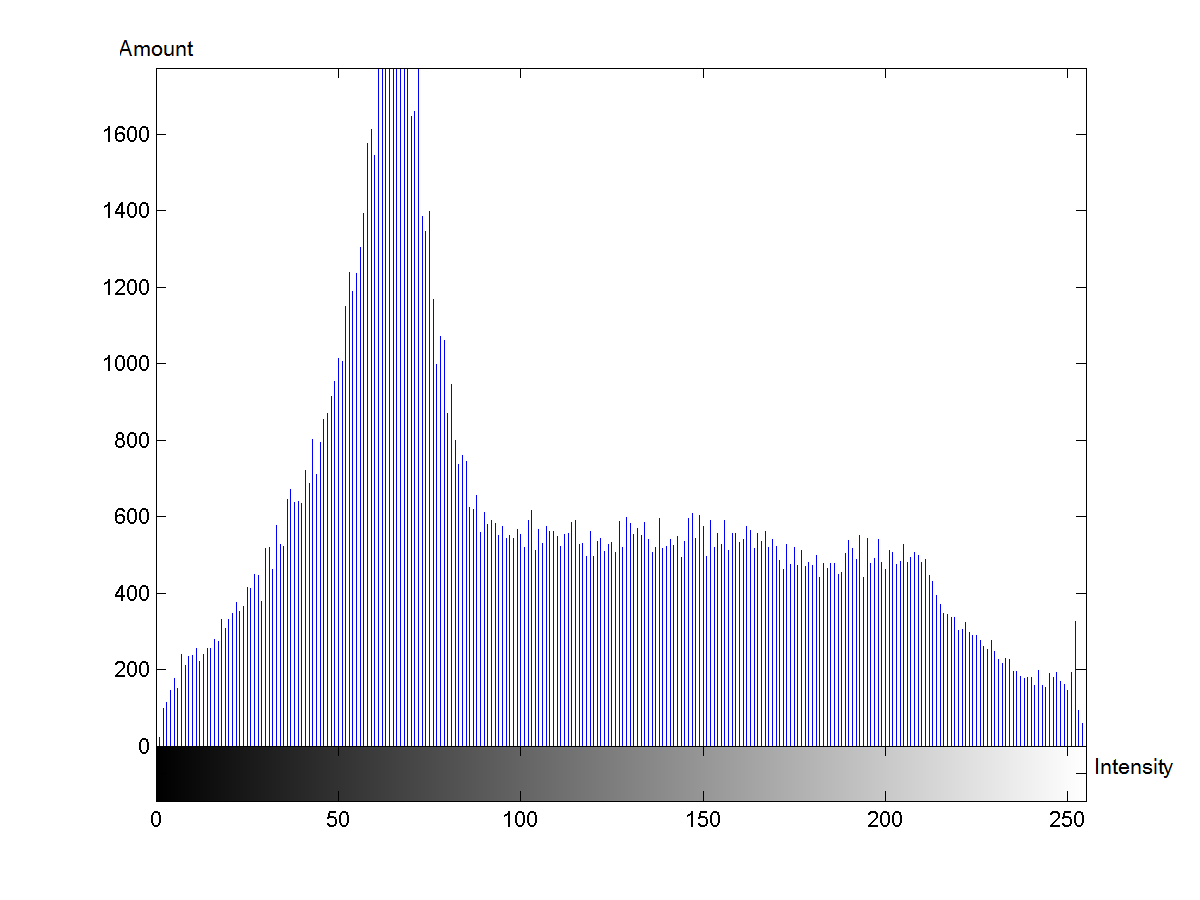
\includegraphics[width=\textwidth]{f3012b.png}
		\caption{}\label{fig:f3012b}
	\end{subfigure}
	\caption{(a) Histogram of gray-scale image (b) Histogram of enhancing the contrast of the gray-scale image}\label{fig:f3012}
\end{figure}

%------------------------------------------------------------------
%	SECTION 5
%------------------------------------------------------------------

\section{Binary Image Conversion}\label{sec:3.5}
This technique uses to convert gray-scale image to binary image. The binary image is a digital image which has only two possible values, i.e. a 1 or 0 for each pixel. Consider Figure \ref{fig:f3013a}, an input image will be converted to binary image. It has intensity values in rang [0, 255]. Next step, a threshold value is assigned in range [0, 1] which is decimal number. The output image then replaces all pixels with luminance greater than threshold value with the value 1, white color, and replaces all other pixels with the value 0, black color,. Specify level in the range [0, 1]. The converted image is shown in Figure \ref{fig:f3013b}.
\begin{figure}
	\centering
	\begin{subfigure}[b]{0.3\textwidth}
		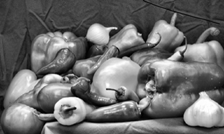
\includegraphics[width=\textwidth]{f3011b.png}
		\caption{}\label{fig:f3013a}
	\end{subfigure}
	\begin{subfigure}[b]{0.3\textwidth}
		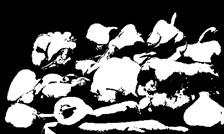
\includegraphics[width=\textwidth]{f3013b.png}
		\caption{}\label{fig:f3013b}
	\end{subfigure}
	\caption{(a) Enhancing the contrast of the gray-scale image (b) Converting the binary image }\label{fig:f3013}
\end{figure}

%------------------------------------------------------------------
%	SECTION 6
%------------------------------------------------------------------

\section{Edge Detection}
Edge detection method is a method to find edges in the gray-scale image by taking a gray-scale or a binary image as its input, and returns a binary image of the same size as one, with 1's where the function finds edges in gray-scale and 0's elsewhere. It is used for image segmentation and data extraction in areas such as image processing, computer vision, and machine vision. Note that, edge is a set of connected curves which indicate the boundaries of objects. Typically, there is corner detection algorithms follow:
\begin{itemize}
	\item{\textbf{Sobel Method:} This method finds edges using the Sobel approximation to the derivative. It returns edges at those points where the gradient of gray-scale image is maximum. The gradient is computed with 3x3 kernels in horizontal $G(y)$ and vertical $G(x)$.\\
		$G(y) = \begin{bmatrix}
			-1 & 0 & 1\\
			-2 & 0 & 2\\
			-1 & 0 & 1
		\end{bmatrix}
		G(x) =\begin{bmatrix}
			1 & 2 & 1\\
			0 & 0 & 0\\
			-1 & -2 & -1
		\end{bmatrix}$
		 }
	\item{\textbf{Prewitt Method:} This method finds edges using the Prewitt approximation to the derivative. It returns edges at those points where the gradient of gray-scale image is maximum. The gradient is computed with 3x3 kernels in horizontal $G(y)$ and vertical $G(x)$.\\
			$G(y) = \begin{bmatrix}
				-1 & 0 & 1\\
				-1 & 0 & 1\\
				-1 & 0 & 1
			\end{bmatrix}
			G(x) =\begin{bmatrix}
				-1 & -1 & -1\\
				0 & 0 & 0\\
				1 & 1 & 1
			\end{bmatrix}$
		}
	\item{\textbf{Roberts Method:} This method finds edges using the Roberts approximation to the derivative. It returns edges at those points where the gradient of gray-scale image is maximum.The gradient is computed with 2x2 kernels in horizontal $G(y)$ and vertical $G(x)$.\\
			$
			G(y) =\begin{bmatrix}
			0 & 1\\
			-1 & 0
			\end{bmatrix}
			G(x) = \begin{bmatrix}
			1 & 0 \\
			0 & -1\\
			\end{bmatrix}$
		}
	\item{\textbf{Laplacian Method:} This is Gaussian method finds edges by looking for zero crossings after filtering gray-scale image with a Laplacian of Gaussian filter.}
	\item{\textbf{Zero-cross Method:} This method finds edges by looking for zero crossings after filtering gray-scale image with a filter you specify.}
	\item{\textbf{Canny Method:} This method finds edges by looking for local maxima of the gradient of gray-scale image. The gradient is calculated using the derivative of a Gaussian filter. The method uses two thresholds, to detect strong and weak edges, and includes the weak edges in the output only if they are connected to strong edges. This method is therefore less likely than the others to be fooled by noise, and more likely to detect true weak edges.}
\end{itemize}

For example, Figure \ref{fig:f3014a} is an input gray-scale image. After using methods of edge detection algorithms, i.e. sobel, prewitt, roberts, laplacian of Gaussian, zero-cross, and canny. The output images are shown in Figure \ref{fig:f3014b} - \ref{fig:f3014g} respectively.
\begin{figure}
	\centering
	\begin{subfigure}[b]{0.4\textwidth}
		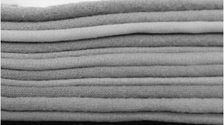
\includegraphics[width=\textwidth]{f3014a.png}
		\caption{}\label{fig:f3014a}
	\end{subfigure}
	\begin{subfigure}[b]{0.4\textwidth}
		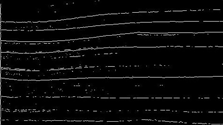
\includegraphics[width=\textwidth]{f3014b.png}
		\caption{}\label{fig:f3014b}
	\end{subfigure}
	\begin{subfigure}[b]{0.4\textwidth}
		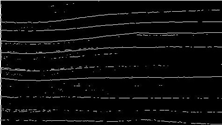
\includegraphics[width=\textwidth]{f3014c.png}
		\caption{}\label{fig:f3014c}
	\end{subfigure}
	\begin{subfigure}[b]{0.4\textwidth}
		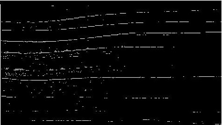
\includegraphics[width=\textwidth]{f3014d.png}
		\caption{}\label{fig:f3014d}
	\end{subfigure}
	\begin{subfigure}[b]{0.4\textwidth}
		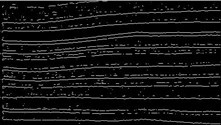
\includegraphics[width=\textwidth]{f3014e.png}
		\caption{}\label{fig:f3014e}
	\end{subfigure}
	\begin{subfigure}[b]{0.4\textwidth}
		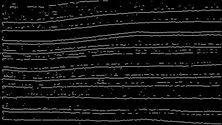
\includegraphics[width=\textwidth]{f3014f.png}
		\caption{}\label{fig:f3014f}
	\end{subfigure}
	\begin{subfigure}[b]{0.4\textwidth}
		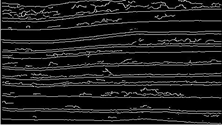
\includegraphics[width=\textwidth]{f3014g.png}
		\caption{}\label{fig:f3014g}
	\end{subfigure}
	\caption{(a) Gray-scale image (b) Sobel image(c) Prewitt image (d) Roberts image(e) Laplacian of Gaussian image (f) Zero-cross image (g) Canny image }\label{fig:f3014}
\end{figure}

All the basic knowledge presented in this chapter will be applied to the work of sheet of cloths counting in the later chapter.